\chapter{Code for Computational Fluid Dynamics}
\label{App:cfd}
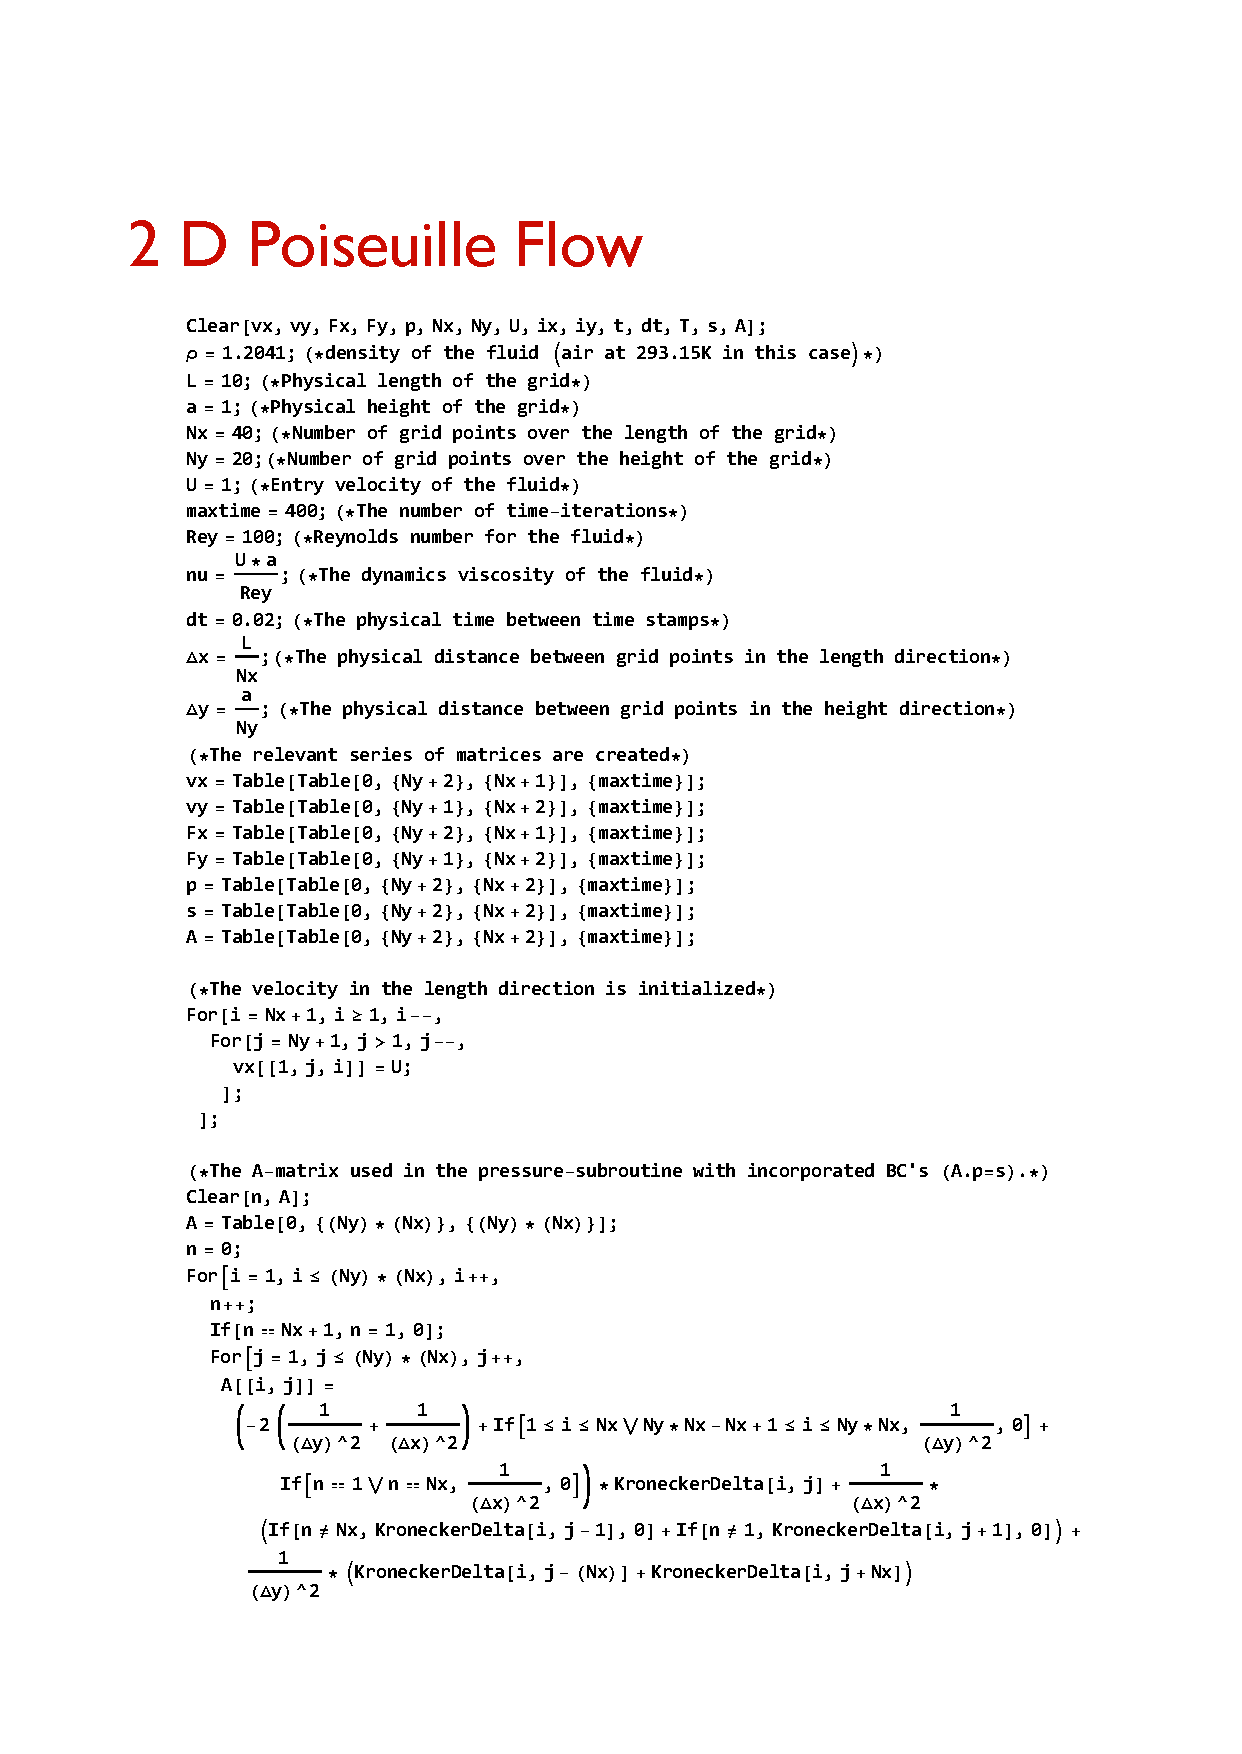
\includepdf[pages=-]{figures/2DPoiseuille.pdf}
\begin{frame}
	%	\frametitle{Forward Kinematics}	
	
	\begin{center}
		\includemedia[
		activate=onclick,
		width=0.75\textwidth
		]{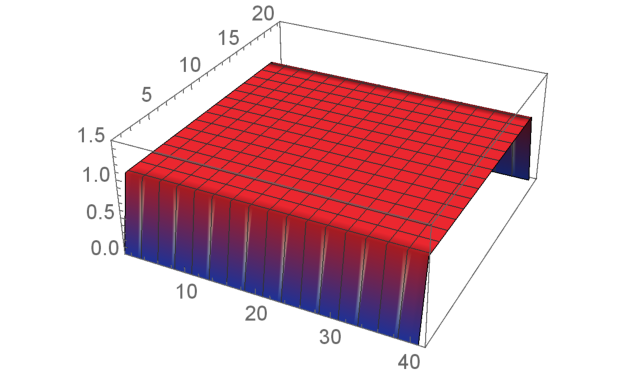
\includegraphics{figures/screensaver.pdf}}{figures/flow2.swf}
	\end{center}
\end{frame}

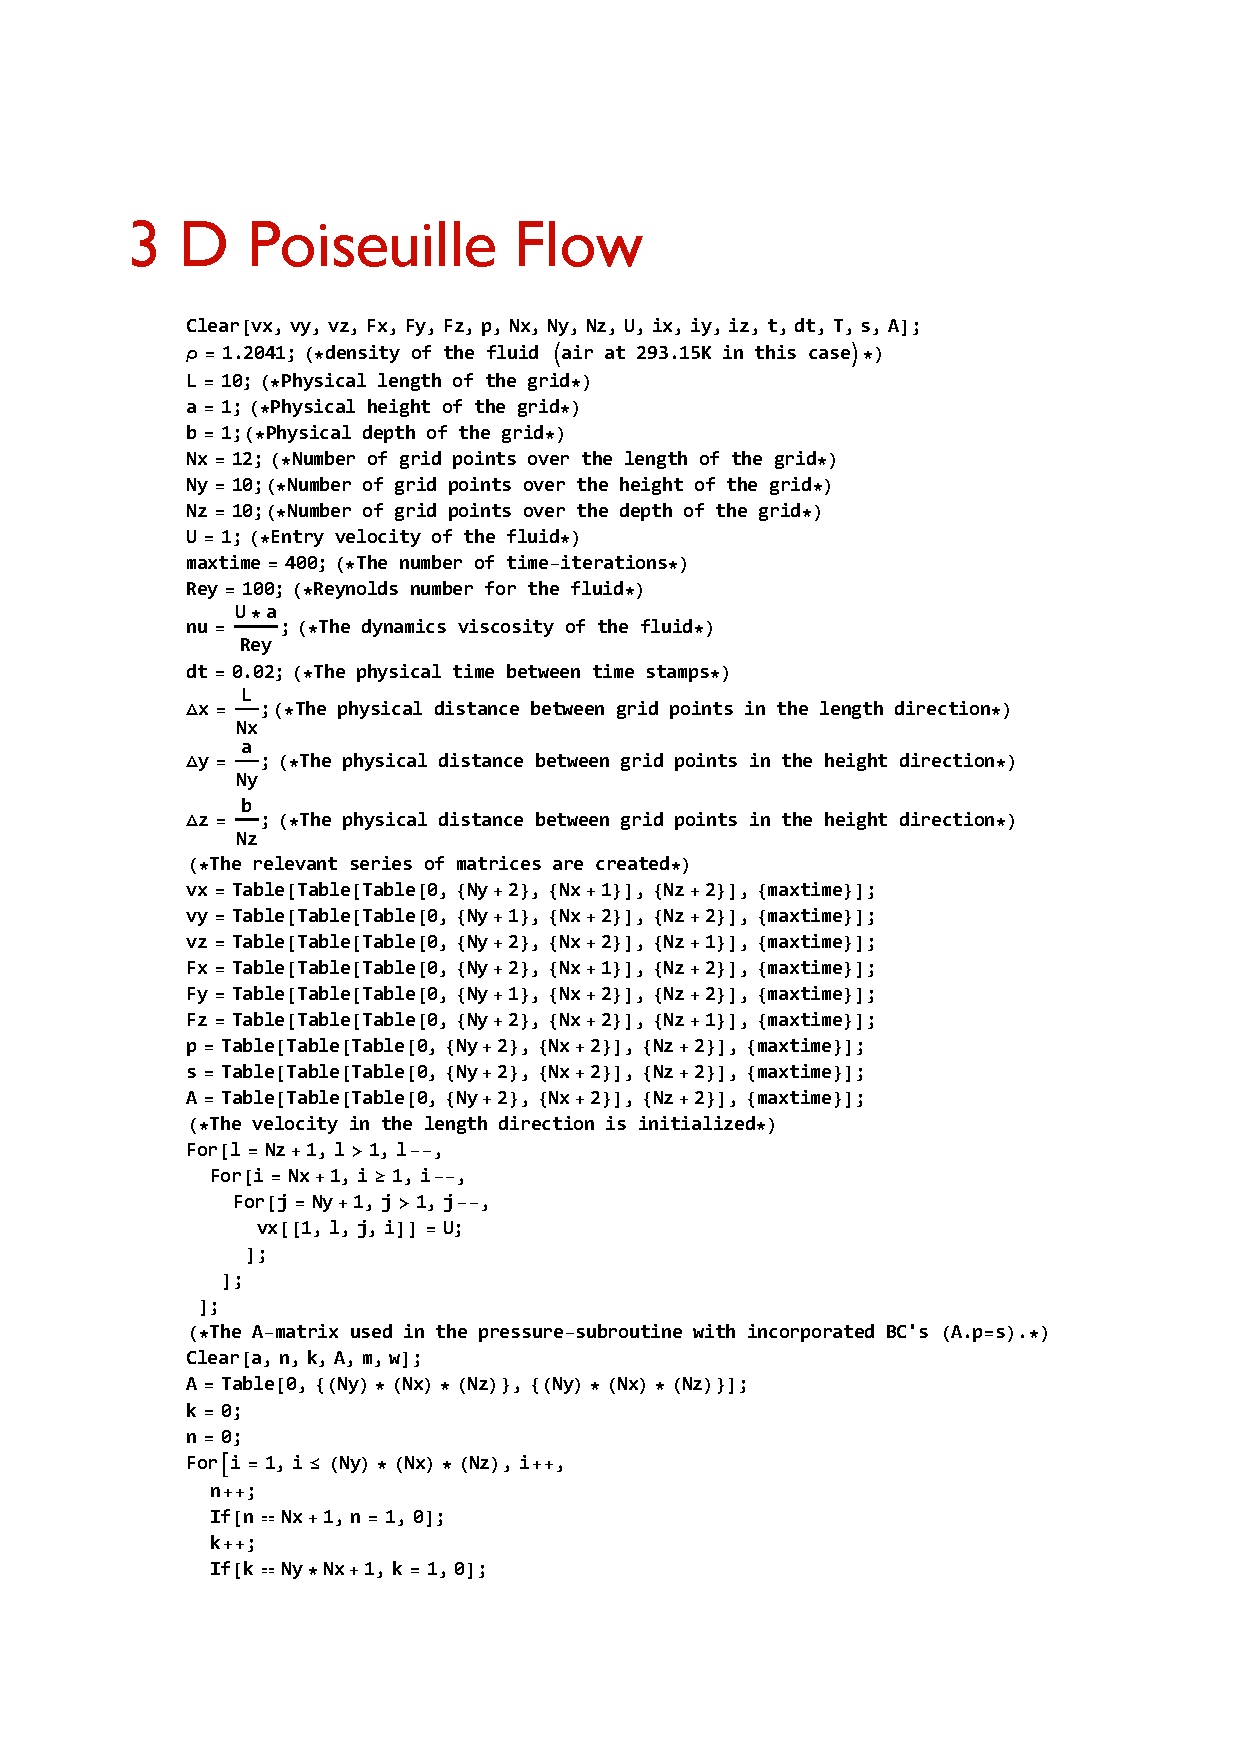
\includepdf[pages=-]{figures/3DPoiseuille.pdf}

\begin{figure}[H]
	\centering
	\captionsetup{width=1\textwidth}
	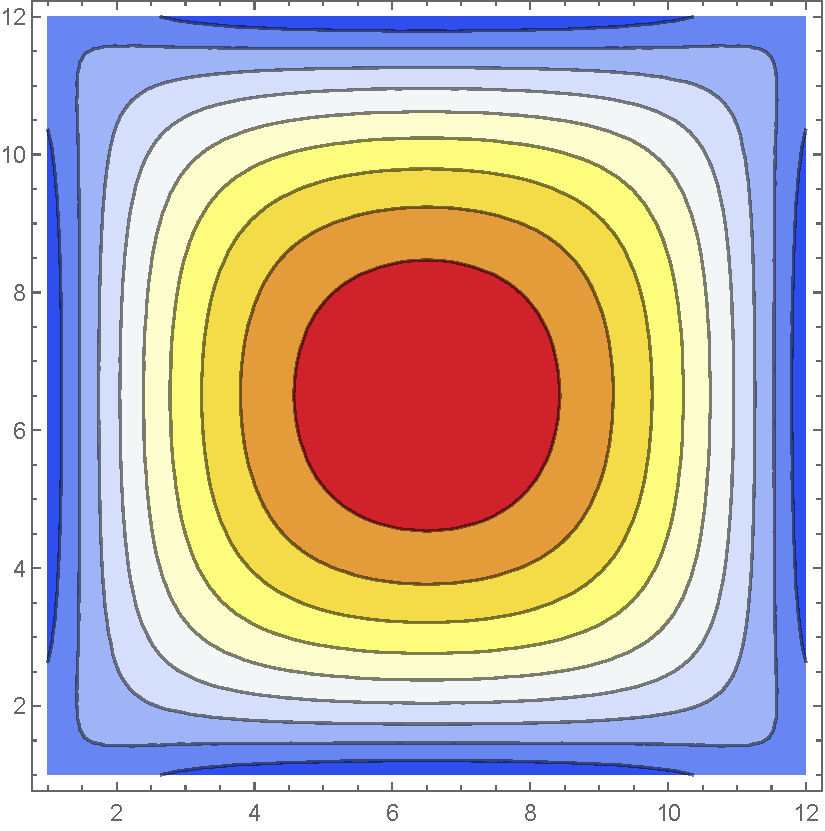
\includegraphics[width=0.3\textwidth]{figures/3D1.pdf}
	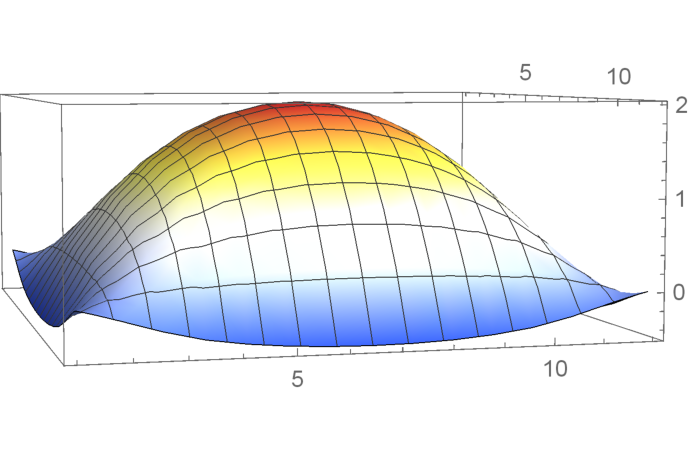
\includegraphics[width=0.3\textwidth]{figures/3D2.pdf}
	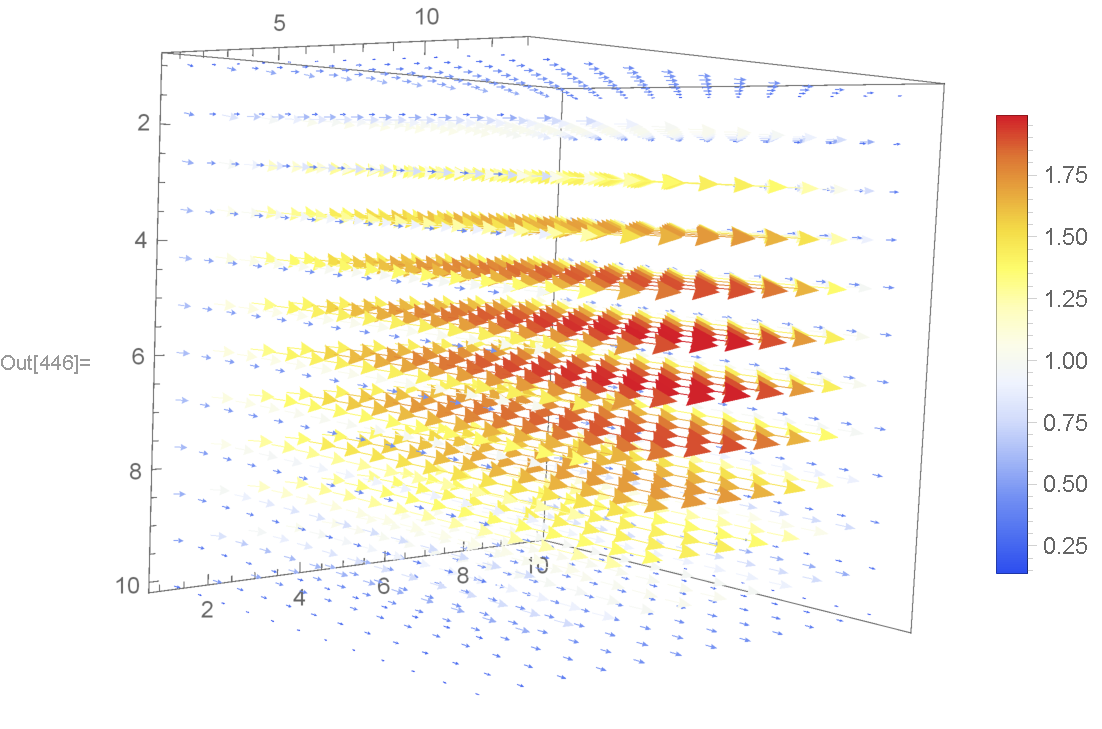
\includegraphics[width=0.3\textwidth]{figures/3D3.pdf}
	\caption
	{Left: A contour plot of the 2D slice of the flow velocity in the length direction at about halfway in the flow direction (the $x$-direction). Middle: A 3D plot of the 2D slice of the flow velocity in the length direction at the end of the channel. The height signify the value of the velocity field in the length direction. Right: A 3D vector plot of the velocity field in the channel.}
\end{figure}


\begin{frame}
	%	\frametitle{Forward Kinematics}	
	
	\begin{center}
		\includemedia[
		activate=onclick,
		width=0.75\textwidth
		]{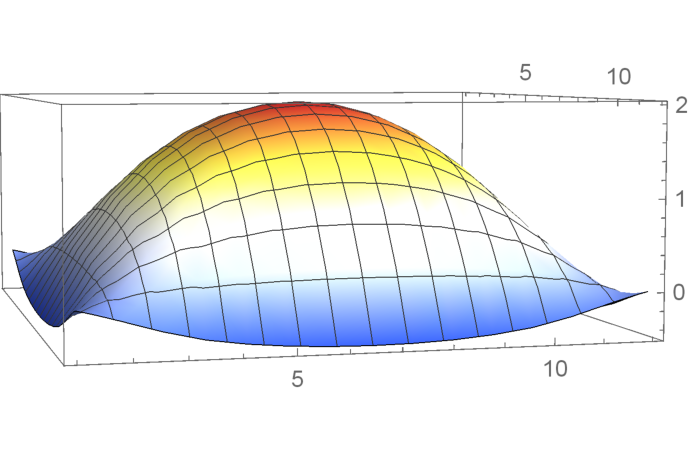
\includegraphics{figures/3D2.pdf}}{figures/flow3.swf}
	\end{center}
\end{frame}

The Navier-Stokes equations (equation \eqref{N6}) are not solve-able in the general case, and so approximations obtained from the physical scenario under consideration must be used in order to apply Navier-Stokes equations. 